%-------------------------------------------------------
%	DOCUMENT CONFIGURATIONS
%-------------------------------------------------------

%-------------------------------------------------------
%	START OF ARCHITECTURE ANALYSE
%-------------------------------------------------------
\subsection{Architecture}
While doing research, the concept and based had to be pretty clear to help us focus on the right track. We then made an architecture for the project. Of course this architecture is not definitive, put helps to understand what we are trying to do. The latest global architecture version can be found on figure ~\ref{img:latest-architecture} in the annexes.

\begin{figure}[htpb]
\centering
\begin{adjustbox}{center}
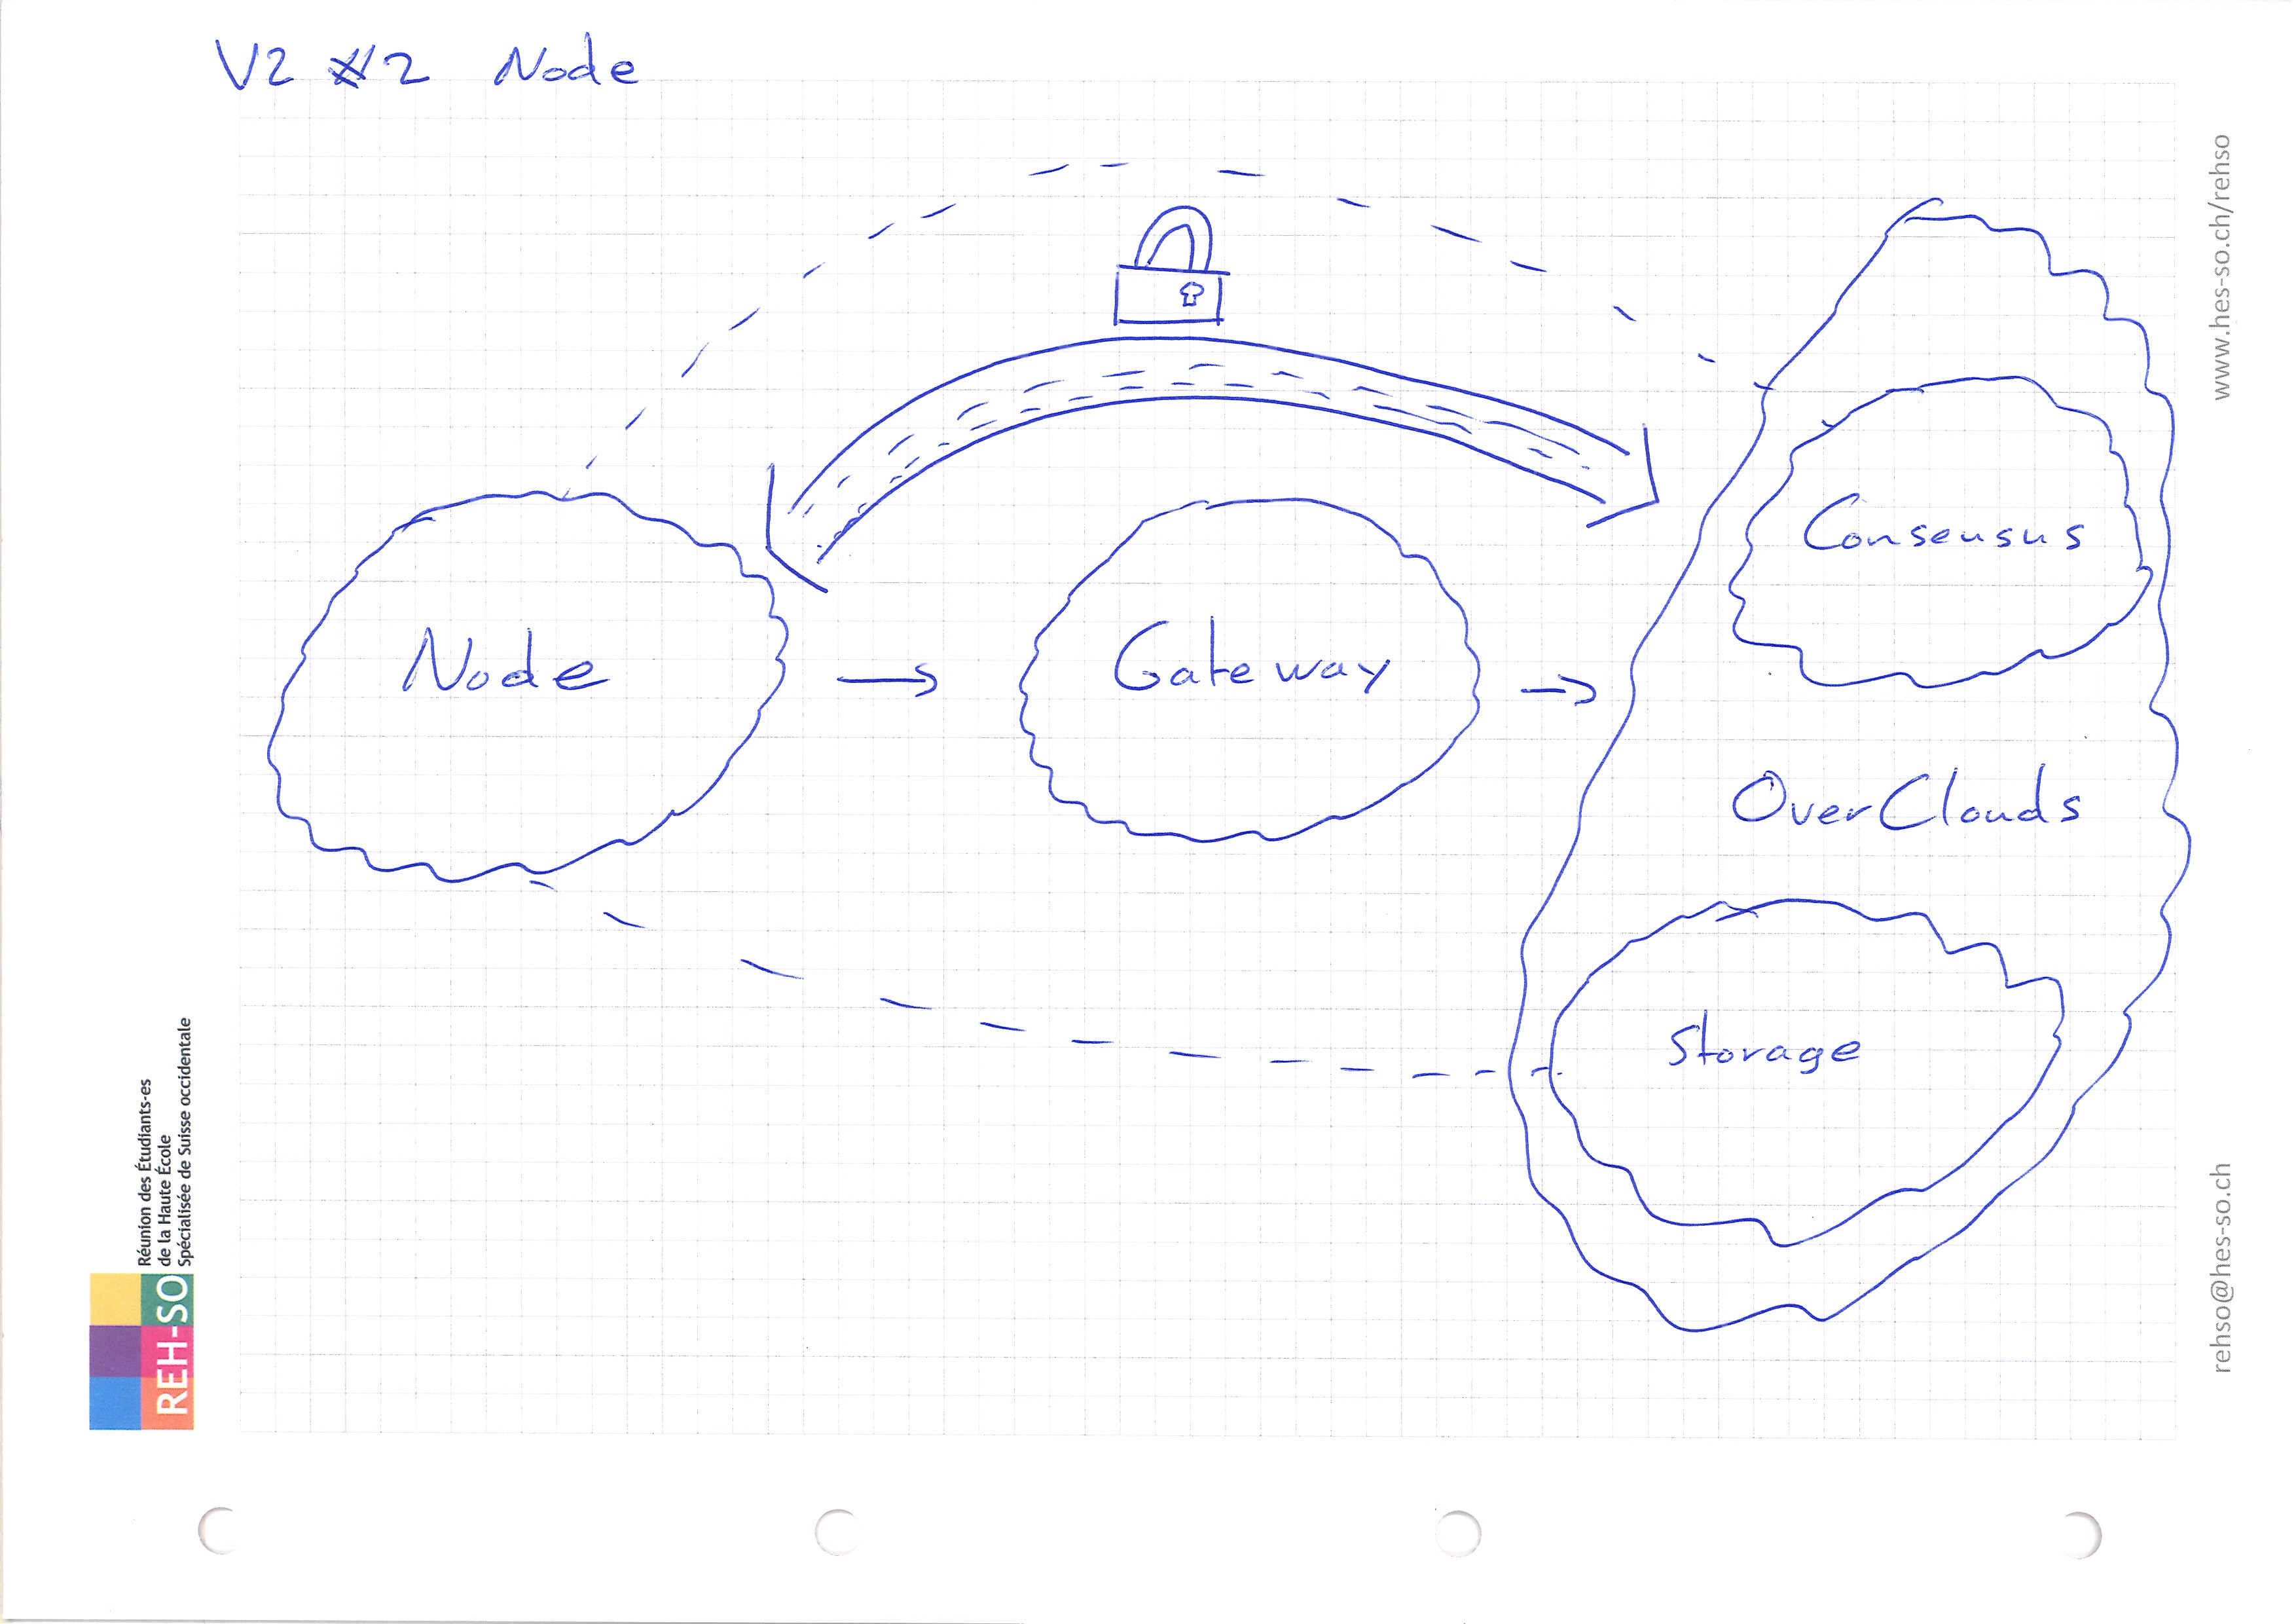
\includegraphics[scale=0.18]{annexes/concepts/Architecture-Draft-global-view-idea-2-node.jpeg}
\end{adjustbox}
\caption{Latest schematic architecture version seen from a User.
\label{img:latest-schematic-architecture-user}}  
\end{figure}

\begin{figure}[htpb]
\centering
\begin{adjustbox}{center}
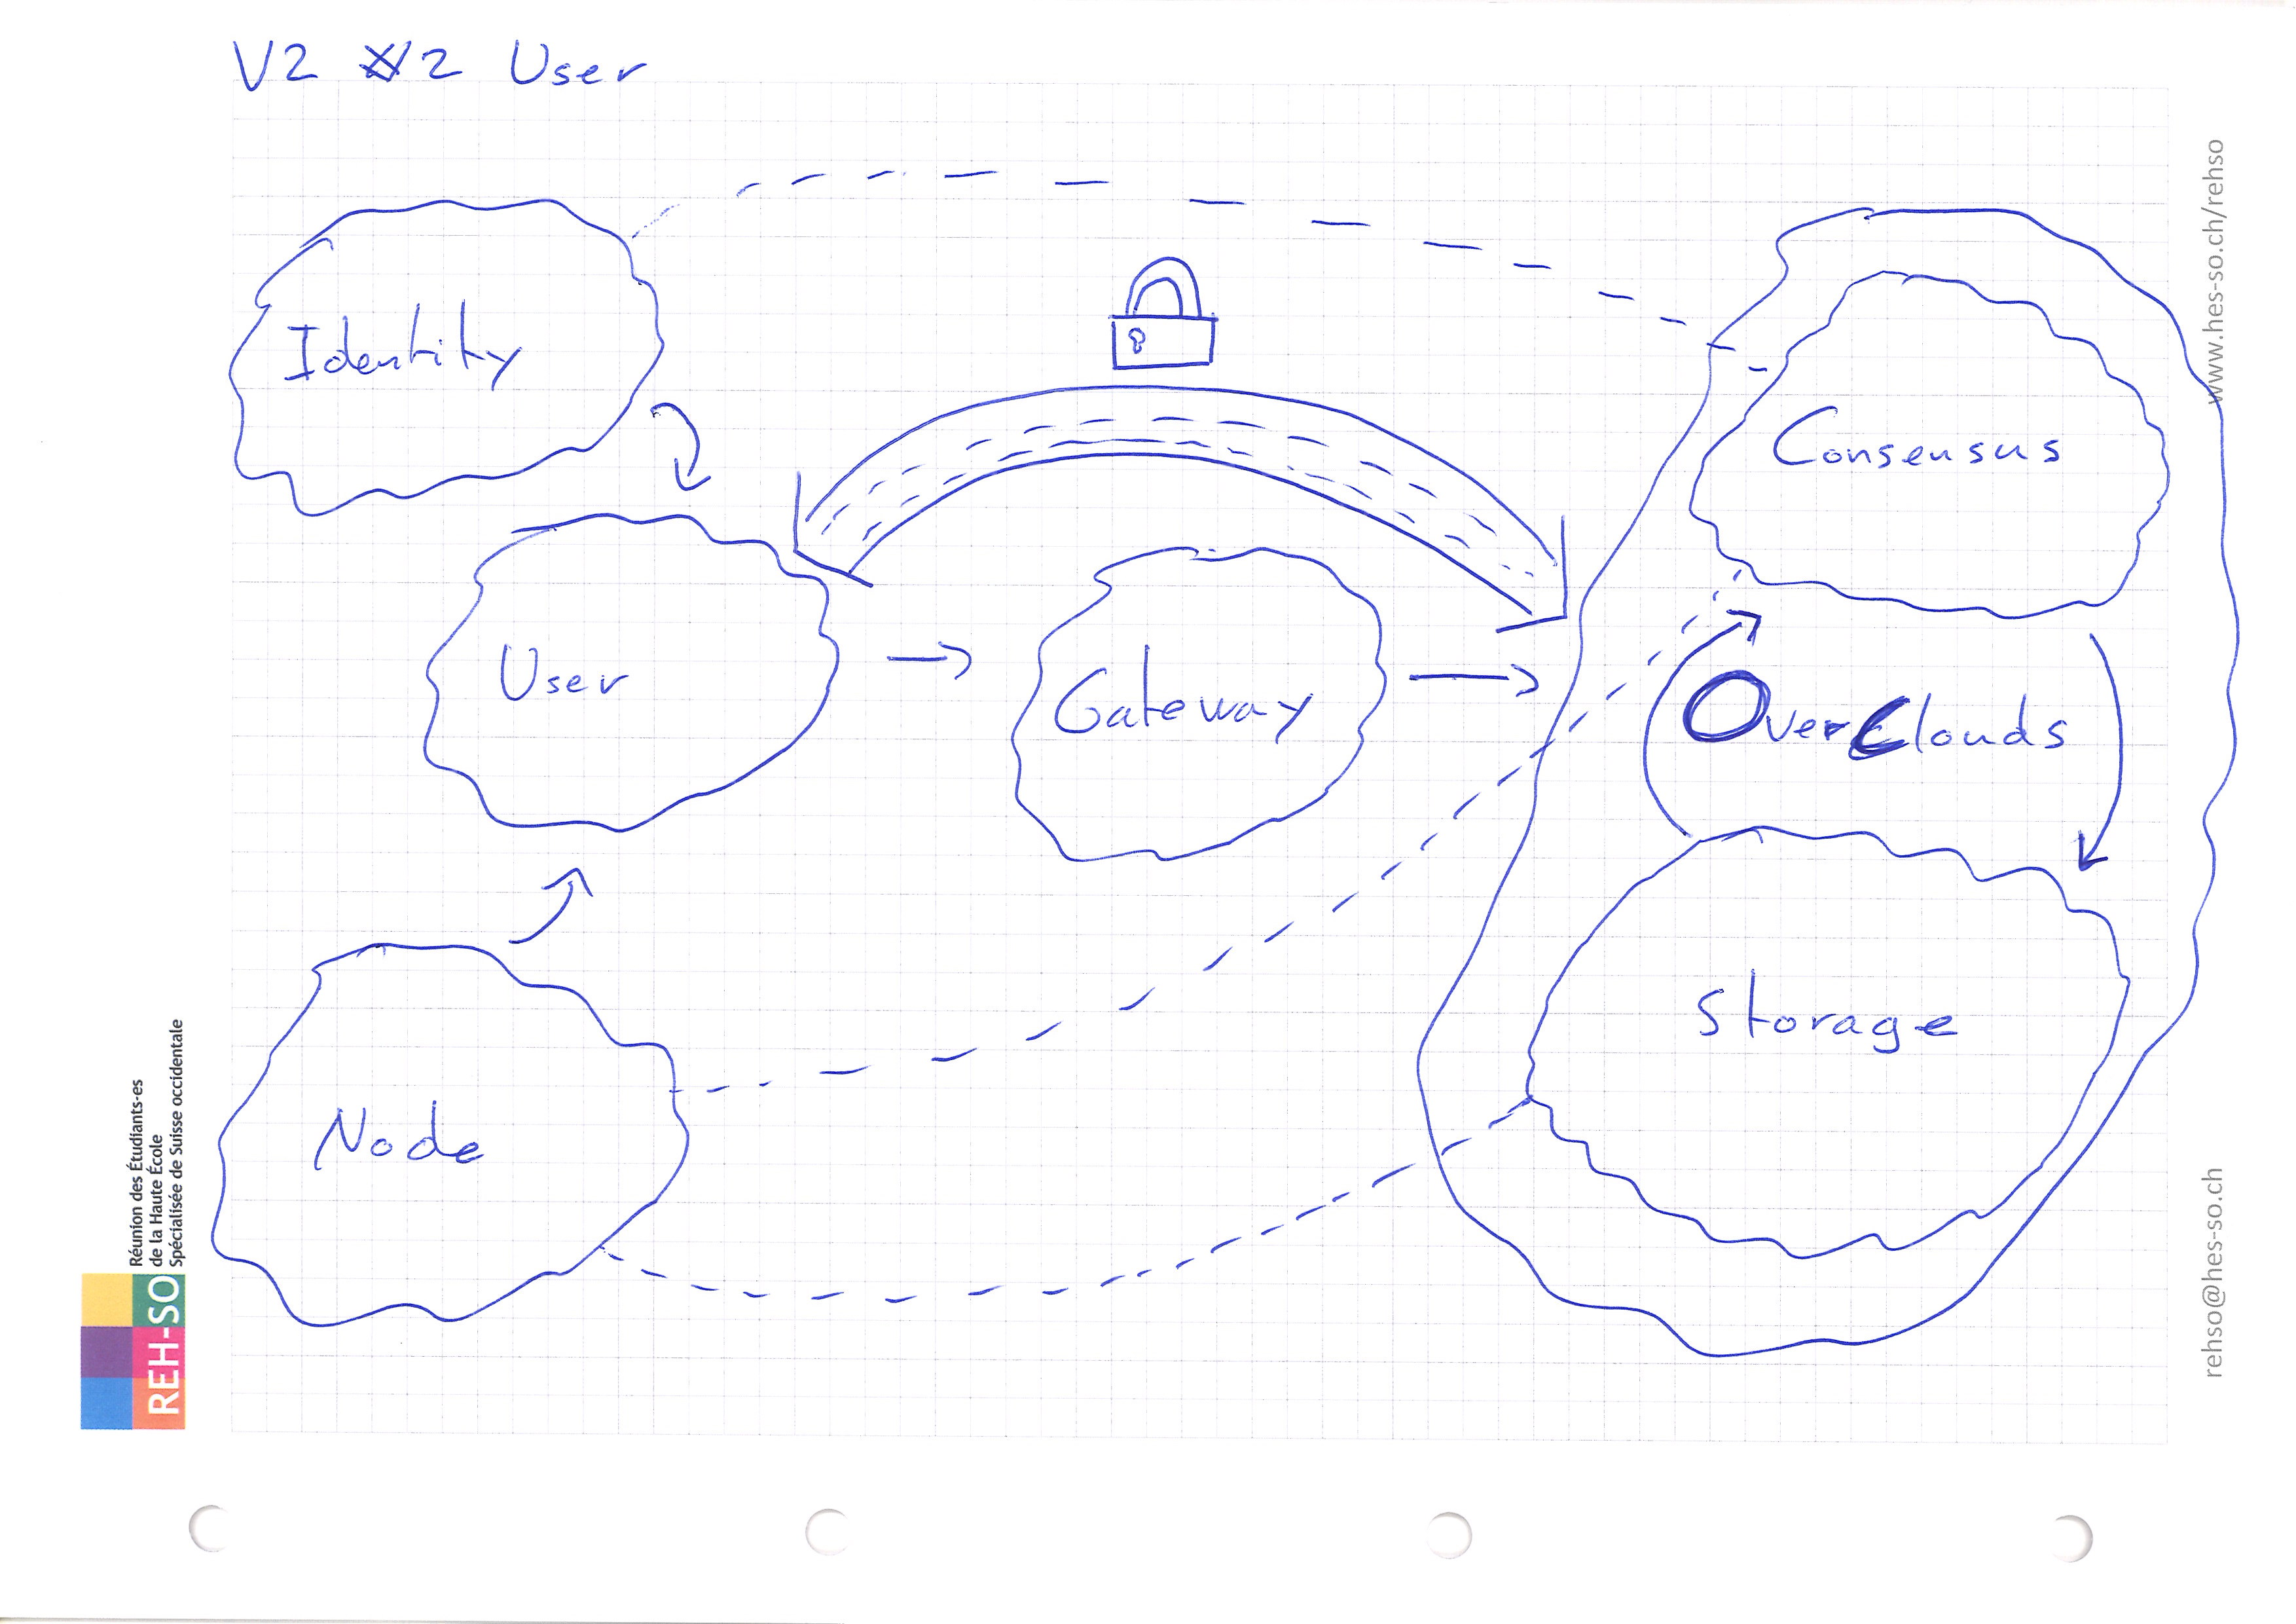
\includegraphics[scale=0.15]{annexes/concepts/Architecture-Draft-global-view-idea-2.jpeg}
\end{adjustbox}
\caption{Latest schematic architecture version seen from a Node.
\label{img:latest-schematic-architecture-node}}  
\end{figure}


%-------------------------------------------------------
%	END OF ARCHITECTURE ANALYSE
%-------------------------------------------------------